%------------------------------------------------------------------------------
% Manuscript for Journal of Applied Crystallography, prepared with the IUCr
% LaTeX macro package (iucr.cls).  Compile with pdflatex.
%------------------------------------------------------------------------------
\documentclass[preprint,pdf]{iucr}          % DO NOT DELETE THIS LINE
\journalcode{J}

\usepackage{amsmath,amssymb}
\usepackage{booktabs}
\usepackage{graphicx}

% --- notation -----------------------------------------------------------------
\newcommand{\Ang}{\text{\AA}}
\newcommand{\Gmet}{\mathbf{G}}
\newcommand{\Pop}{\mathbf{P}}
\newcommand{\Uop}{\mathbf{U}}
\newcommand{\Mop}{\mathbf{M}}
\newcommand{\Bbasis}{\mathbf{B}}
\newcommand{\Cmat}{\mathbf{C}}
\newcommand{\sortkey}{\mathbf{s}}
\newcommand{\Sclosure}{\mathcal{S}}
\newcommand{\tr}{\operatorname{tr}}
\newcommand{\sort}{\operatorname{sort}}
\newtheorem{lemma}{Lemma}

% --- computational-check marks -------------------------------------------------
% Every checkable statement carries \chk{label}; the mark prints [S.n], where n is
% the number of the corresponding entry in the Supporting Information
% (zwart_selling_closure_SI.tex).  The mapping below is the single place where the
% numbering is fixed; the SI carries the same labels in the same order.
\makeatletter
\newcommand{\chk}[1]{\textsuperscript{[S\@nameuse{zn@#1}]}}
\@namedef{zn@z:reduction-step}{1}
\@namedef{zn@z:closure-count}{2}
\@namedef{zn@z:type-rule}{3}
\@namedef{zn@z:pdb-types}{4}
\@namedef{zn@z:one-key}{5}
\@namedef{zn@z:trajectory}{6}
\@namedef{zn@z:lowerbound}{7}
\@namedef{zn@z:euclid}{8}
\@namedef{zn@z:fibre}{9}
\@namedef{zn@z:d7}{10}
\@namedef{zn@z:noise}{11}
\@namedef{zn@z:stabilise}{12}
\@namedef{zn@z:floor-invariance}{13}
\@namedef{zn@z:coset}{14}
\@namedef{zn@z:reindex-proc}{15}
\@namedef{zn@z:coset-reps}{16}
\@namedef{zn@z:pseudo}{17}
\@namedef{zn@z:verify-tol}{18}
\@namedef{zn@z:noisy-frames}{19}
\@namedef{zn@z:lepage}{20}
\@namedef{zn@z:reindex-bench}{21}
\@namedef{zn@z:brute-complete}{22}
\@namedef{zn@z:timing}{23}
\@namedef{zn@z:embedding}{24}
\@namedef{zn@z:audit}{25}
\@namedef{zn@z:effrank}{26}
\@namedef{zn@z:lysozyme}{27}
\@namedef{zn@z:xfel}{28}
\makeatother

\begin{document}                  % DO NOT DELETE THIS LINE

\title{Selling reduction and sorted Kurlin roots: a conservative Euclidean key for lattice search and exact reindexing}
\shorttitle{Selling reduction and sorted Kurlin roots}

\cauthor{Petrus H.}{Zwart}{phzwart@lbl.gov}{}
\aff{Molecular Biophysics and Integrated Bioimaging Division, Lawrence Berkeley National Laboratory, 1 Cyclotron Road, Berkeley, CA 94720, \country{USA}}
% ORCID: not inserted. A public ORCID search did not return a record that
% could be verified as this author (0000-0002-1539-0297 is a different person).
\shortauthor{Zwart}

\keyword{lattice reduction}\keyword{Selling reduction}\keyword{obtuse superbase}\keyword{lattice isometry}\keyword{reindexing}\keyword{nearest-neighbour search}\keyword{serial crystallography}\keyword{Protein Data Bank}

\maketitle                        % DO NOT DELETE THIS LINE

\begin{synopsis}
A unit cell is one description of a lattice, not the lattice itself. A six-number key built from the sorted square roots of the Selling scalars gives every basis of a lattice the same continuous coordinate, whose Euclidean distance never exceeds the true lattice distance, so ordinary nearest-neighbour software can retrieve candidate matches safely; the finite set of obtuse superbases then decides identity exactly and returns the integer reindexing operator with its full symmetry coset.
\end{synopsis}

\begin{abstract}
Every crystallographic unit cell is a choice of basis for a lattice, and a lattice has infinitely many bases. Classical reduction (Niggli, Buerger, Delone) selects one representative cell per lattice, which suits tabulation and lattice typing but not comparison: an arbitrarily small change to a lattice can make its representative jump. Searching archives of hundreds of thousands of cells, following lattices through thousands of serial-crystallography frames, and tracing a lattice along a perturbation trajectory are comparison tasks, and they need a coordinate that does not jump. This paper separates the work into two stages with different representations. For search, each lattice receives a single vector of six numbers, the square roots of the six Selling scalars of its obtuse superbase sorted into increasing order; these are Kurlin's root products with their pairing discarded. The key varies continuously with the lattice, is identical for every basis of the lattice at every Voronoi type, and is indexed with a standard KD tree. It is deliberately not unique --- a bounded number of distinct lattices can share a key --- but its Euclidean distance is a lower bound on the orbit distance between lattices, so a radius query cannot miss a match. For certification, the candidates are compared exactly: the finite set of obtuse superbases of each lattice, here called the Selling closure, is enumerated and an integer change-of-basis matrix is constructed from retained integer coordinates and verified against the metric tensor. Nothing is rounded, and symmetry-related alternatives are returned as a coset rather than lost. The two stages are used to index 206\,214 PDB cells, to place archival hen egg-white lysozyme cells on a common shape trajectory, to decompose per-crystal cell variation in a 12\,474-crystal XFEL data set, and to replace a 6960-matrix reindexing search by a cached two-operator coset. The rule throughout is to search continuously and conservatively and to decide exactly.
\end{abstract}

%==============================================================================
\section{Introduction}
%==============================================================================

A lattice is a set of points. A unit cell describes that set by three vectors $v_1,v_2,v_3$, and the metric tensor $\Gmet=\Bbasis^{\mathsf T}\Bbasis$ collects their lengths and angles. Any integer matrix $\Mop$ of determinant $\pm1$ produces another equally valid cell for the same lattice, $\Bbasis'=\Bbasis\Mop$ and $\Gmet'=\Mop^{\mathsf T}\Gmet\Mop$, so a lattice is not one metric tensor but an infinite family of them.

The traditional way to remove the ambiguity is reduction: a rule that selects one cell from the family. Niggli reduction (Niggli, 1928; Grosse-Kunstleve \emph{et al.}, 2004) is the standard example, and for its original purposes --- reporting a cell, assigning a Bravais type, looking a cell up in a table --- it is exactly right. It has one unavoidable side effect. A rule that picks one representative must decide what to do at the boundaries where two representatives are equally good, and at those boundaries the chosen cell changes abruptly while the lattice changes smoothly.\chk{z:trajectory} The lattice is continuous; the coordinate assigned to it is not. For classification this rarely matters. For comparison it matters constantly: to ask how close two lattices are across an archive, across the frames of a serial experiment, or along a heating or dehydration series, one needs a coordinate that moves a little when the lattice moves a little.

There is a second, less obvious demand. A comparison coordinate necessarily discards basis information, but reindexing --- transforming Miller indices, coordinates or symmetry operators from one cell setting to another --- needs that information back, and needs it exactly. A method that compares well but reindexes approximately is of limited use in a crystallographic pipeline.

The proposal made here is not to find one representation that does both jobs, but to stop asking for one. Search is done on a coarse, continuous, Euclidean key; certification and reindexing are done exactly on a finite basis-aware object; and the hand-off between them is made safe by a one-sided distance bound. The ingredients are classical or recent, and the paper is explicit about which is which. Selling reduction and the obtuse superbase go back to Selling, Delone and Bravais (Bravais, 1850; Delone, 1932), the conorm/vonorm language is that of Conway \& Sloane (1992), and the crystallographic $S^6$ embedding, the uniqueness of the reduced Selling scalars as a list and the practical reduction algorithm are due to Andrews, Bernstein and Sauter (Andrews \& Bernstein, 1988, 2014, 2016, 2023; Andrews \emph{et al.}, 2019). The type-dependent enumeration of obtuse superbases, the completeness proof of the resulting isometry classification and the perturbation bound on individual root products are Kurlin's (Bright \emph{et al.}, 2021; Kurlin, 2026). What is added here is elementary: the observation that sorting the six root products gives one key per lattice at every Voronoi type, a lemma that its Euclidean distance is a lower bound on the orbit distance, a noise analysis at symmetric lattices, and an exact reindexing procedure over the complete finite set of obtuse superbases --- the \emph{Selling closure} --- that returns the automorphism coset without a symmetry tolerance. The main text keeps to the constructions and the results; derivations and proofs are in Appendices~A--D, and every statement that can be checked by computation carries a mark $^{[\mathrm{S}n]}$ pointing at the corresponding check in the Supporting Information.

%==============================================================================
\section{Theory and methods}
%==============================================================================

\subsection{Obtuse superbases and the Selling closure}
\label{sec:closure}

Selling reduction (Appendix~A) turns the infinite family of cells into a finite one. Adding a fourth vector $v_0=-(v_1+v_2+v_3)$ gives a \emph{superbase}, four vectors that sum to zero; reduction adjusts them until every pair meets at a right or obtuse angle. The six \emph{conorms} $p_{ij}=-v_i\cdot v_j\ge0$ of an obtuse superbase are the negatives of the Selling scalars of Andrews \emph{et al.} (2019). For a generic lattice the obtuse superbase is unique up to relabelling the four vectors and negating all of them --- 24 relabellings, 48 with the sign.\chk{z:closure-count}

For symmetric lattices this is no longer true. Kurlin (2026) shows that the obtuse superbase is unique up to relabelling only when the Voronoi cell of the lattice is the generic truncated octahedron (type V1); for the four degenerate types V2--V5, further obtuse superbases exist that are not relabellings of one another, obtained from the reduced one by a Selling move at a conorm that is exactly zero. An orthorhombic P lattice, for example, has 32 obtuse superbases (counted as unordered sets of four vectors, the superbase and its global negation being distinct) falling into four families.\chk{z:closure-count} The complete finite set of obtuse superbases of a lattice $\Lambda$ is called here its \emph{Selling closure} $\Sclosure(\Lambda)$; Table~\ref{tab:closure} gives its size and structure by Voronoi type, and Appendix~A gives the rule that reads the type off the zero pattern of the reduced conorms.\chk{z:type-rule} Two facts matter for what follows. The closure is finite, so it can be enumerated. And the classical statement that it consists of ``24 relabellings'' is correct only for lattices with no symmetry: monoclinic P lattices are V4 and orthorhombic P lattices are V5,\chk{z:pdb-types} so for a large fraction of real cells the shortcut undercounts.

\subsection{The sorted six-number key}
\label{sec:key}

From any obtuse superbase, take the square roots of the six conorms so that they have units of length --- these are Kurlin's root products --- and sort them:
\begin{equation}
\sortkey(\Lambda)=\sort\big(\sqrt{p_{01}},\sqrt{p_{02}},\sqrt{p_{03}},\sqrt{p_{12}},\sqrt{p_{13}},\sqrt{p_{23}}\big)\in\mathbb R^6 .
\label{eq:key}
\end{equation}
Sorting discards which conorm belonged to which pair of vectors, so relabelling the superbase does not change the key; and because every member of the closure carries the same six numbers in some order (Appendix~B), every basis of a lattice yields the same key at every Voronoi type.\chk{z:one-key} Sorting is also continuous, so small changes in the lattice give small changes in the key, including across the boundaries where a reduction rule changes its mind.\chk{z:trajectory} For shape-only comparison the key is divided by $V^{1/3}$.

The key is Euclidean in a substantive sense. Its distance is the quotient distance of $\mathbb R^6$ by \emph{all} permutations of the six entries (Lemma~\ref{lem:lb}), and because that permutation group is generated by reflections the quotient is the convex cone $\{s_1\le\dots\le s_6\}$ with the ordinary flat metric.\chk{z:euclid} The physically exact relabelling group --- the image of $S_4$ in $S_6$ --- is smaller and contains no reflections, so its quotient, the space in which Kurlin's complete invariant lives, is not Euclidean; this is why a metric has to be constructed there separately (Appendix~B). Because the sorted key lives on a flat cone, KD trees, neighbour graphs and principal components apply to it without modification.

What the key is not is a fingerprint. With the pairing gone, a few distinct lattices can share a key: generically 30 for triclinic (V1) lattices, 15 for V2, 4 for V4, and none for V3 and V5 (Appendix~B).\chk{z:fibre} This is harmless provided equality of keys is never used as a proof of identity. The key is a filter, and it is a safe one because of the following statement, proved in Appendix~B.

\begin{lemma}[conservative sorted-key distance]
\label{lem:lb}
Let $x,y\in\mathbb R^6$ and let $G\subseteq S_6$ be any set of permutations. Then
\begin{equation}
\|\sort(x)-\sort(y)\|_2=\min_{\sigma\in S_6}\|x-\sigma y\|_2\le\min_{\sigma\in G}\|x-\sigma y\|_2 .
\end{equation}
\end{lemma}

With $G$ the image of $S_4$, the key distance is a lower bound on the true orbit distance between two lattices.\chk{z:lowerbound} A radius query on keys therefore returns every lattice within that radius of the query, plus occasionally a few impostors, which the next stage removes. A fixed-$k$ nearest-neighbour query carries no such guarantee, because key collisions can crowd the list; it remains a useful exploratory tool.

\subsection{Noise at symmetric lattices}
\label{sec:noise}

Taking square roots gives the key length units and matches Kurlin's construction, but it has a cost at exactly the lattices that are most common. Where a conorm is zero --- a right angle in the superbase, which every orthorhombic, tetragonal, hexagonal and monoclinic P lattice has --- $\sqrt p$ has infinite slope, so a small angular error produces a disproportionately large change in the key: the key is H\"older-$\tfrac12$ rather than Lipschitz there (Appendix~C). On the CXIDB~83 hexagonal cell a $0.01^\circ$ angular error moves the key by about $1.4$--$1.6$\,\Ang, ten times the $c$-axis spread measured in Section~\ref{sec:xfel}.\chk{z:noise} The remedy is to replace $\sqrt p$ by a monotone map that depends only on the conorm and on lattice invariants, which preserves one-key-per-lattice and Lemma~\ref{lem:lb} in the transformed metric. Appendix~C gives three such maps --- a floored root, a soft threshold and the plain sorted conorms --- and their measured noise reduction.\chk{z:stabilise} The archival key of this paper is the plain $\sqrt p$ of equation~(\ref{eq:key}); the per-frame analysis of Section~\ref{sec:xfel} uses the sorted conorms without the square root.

\subsection{Exact certification and reindexing over the closure}
\label{sec:reindex-proc}

The usual way to reindex a new cell $N$ onto a reference $R$ is to find the metric symmetry of the lattice by a Le~Page-type search (Le Page, 1982): enumerate directions that are twofold axes of the metric to within an angular tolerance, build the point group, and read admissible reindexing operators off it. That procedure answers a different question from the one reindexing asks. It finds operators that are near-symmetries of one metric, which is what pseudo-symmetry and twin-law analysis need; reindexing needs the operator that relates two settings, and the two coincide only when the lattice is exactly symmetric. Away from exact symmetry the relating operator is still an exact integer matrix, but it drops out of the tolerance-enlarged group as the lattice moves away from the symmetric locus (Section~\ref{sec:flip}),\chk{z:lepage} and widening the tolerance admits unrelated pseudo-symmetries instead. Reduction flips make matters worse: a reduced-cell algorithm can hand back $R$ and $N$ in different settings for reasons that have nothing to do with symmetry.

The procedure used here never asks how symmetric the lattice is. It asks only whether an integer basis change maps one metric onto the other, over a finite list of candidates that is complete by construction. Its steps are as follows; Appendix~D gives the pseudo-code and the form of the operator.

\begin{enumerate}
\item \emph{Go primitive, and remember how.} If $R$ or $N$ is given in a centred conventional setting, convert to a primitive basis with the rational centering matrix $\Cmat$, $\Bbasis_{\rm prim}=\Bbasis_{\rm conv}\Cmat$, and keep $\Cmat$. This is the only rational step; everything after it is integer.
\item \emph{Selling-reduce, recording integer coordinates.} Reduce each primitive basis to an obtuse superbase and keep the four superbase vectors as integer triples in the primitive basis ($\Uop_R$, $\Uop_N$).
\item \emph{Enumerate the closure.} From the zero pattern of the conorms, with zeros detected at a tolerance derived from the noise level (Appendix~C), enumerate $\Sclosure(R)$ and $\Sclosure(N)$. For the reference this is done once and cached; it contains at most 32 members.
\item \emph{Optional key screen.} If the sorted keys differ by more than the noise-derived radius, $N$ is not a setting of $R$ and no operator search is needed.
\item \emph{Form every candidate operator.} For each pair of closure members, each of the 24 relabellings and each overall sign, take three of the four superbase vectors as columns of integer matrices $\Uop_R'$, $\Uop_N'$ and set $\Pop=\Uop_R'\,\Uop_N'^{-1}$. Every $\Pop$ is an integer matrix of determinant $\pm1$.
\item \emph{Keep those that carry the metric.} Accept $\Pop$ if $\|\Pop^{\mathsf T}\Gmet(R)\Pop-\Gmet(N)\|$ is below a residual tolerance calibrated on the same noise model as step~3. The residual is linear in the metric.
\item \emph{Report the coset, not one matrix.} The accepted set is $\Pop_0H$ with $H$ the automorphism group of the lattice. Return all of it, separated by determinant sign if handedness matters. Choosing among the members is not a geometric question; intensity statistics decide, or the ambiguity is carried forward. When the space group is known, operators differing by an element of the Laue group $L$ give the same intensities, so the distinct indexing alternatives are the cosets $H/L$, $|H|/|L|$ of them, and one representative per coset is passed to the intensity test (Lebedev \emph{et al.}, 2006; Brehm \& Diederichs, 2014; Gildea \& Winter, 2018).
\item \emph{Propagate.} With $\Bbasis_N=\Bbasis_R\Pop$: fractional coordinates $x_R=\Pop\,x_N$, Miller indices $h_R=\Pop^{-\mathsf T}h_N$, symmetry operators $W_R=\Pop W_N\Pop^{-1}$; in conventional settings $\Pop_{\rm conv}=\Cmat_R\,\Pop\,\Cmat_N^{-1}$, rational with the centering denominators.
\end{enumerate}

Nothing in steps 1--8 is rounded to an integer; the operators are integer because they are built from integer coordinates, and floating point enters only in the comparison of step~6. Symmetry tolerance is not used to find the operator. The one tolerance that remains decides whether two metrics are the same lattice and, at a symmetric locus, how large the coset is (Appendix~D).

Everything that depends on the reference is computed once. For a fixed $R$ the centering matrix, primitive metric, reduced superbase, the complete closure with integer coordinates, the sorted key and its radius, and the automorphism coset $H=\mathrm{Aut}(R)$ obtained by running steps 5--6 of $R$ against itself are cached. The full closure has at most 32 superbases, so the cache is small, and it is exactly the object that the ``24 relabellings'' shortcut omits. A new frame $N$ then costs one Selling reduction, one closure enumeration (needed only if $N$ is itself near a symmetry stratum; otherwise its closure is the single reduced superbase), and at most $32\times|\Sclosure(N)|\times48$ integer $3\times3$ products, each followed by one metric residual. Because $H$ is known in advance, the coset for a frame is reported as $\Pop_0$ times the known $H$, and if the space group is known, as $\Pop_0$ together with $|H|/|L|$ branches --- two for $P6_3$, one for $P4_32_12$ and $P2_12_12_1$ --- which is what an indexing-ambiguity resolver downstream requires.\chk{z:reindex-bench}

\subsection{Pseudo-symmetry as cosets between closures}
\label{sec:pseudo}

The closure yields the exact automorphism group of $R$. Operators that are automorphisms of a nearby, more symmetric lattice --- the source of pseudo-merohedral twinning and of indexing ambiguity near a symmetry stratum --- are not in it, and adding them requires deciding what ``nearby'' means. Table~\ref{tab:ambiguity} separates the four sources of ambiguity in assigning indices and where each is resolved. The reduction flip of Section~\ref{sec:flip} is setting ambiguity; treating it as pseudo-symmetry is what makes a Le~Page gate lose it. At exactly $a=c$ the first two rows of the table merge, because the flip operator becomes an automorphism.

For pseudo-symmetry the nearby equality is imposed and the closure used twice. The lattice $R^*$ on the stratum is built, its closure $\Sclosure(R^*)$ enumerated and self-matched to give $H^*=\mathrm{Aut}(R^*)$. Then $H\subseteq H^*$, the pseudo-symmetry operators are the non-trivial cosets $H^*/H$, and the branches that intensity statistics must examine are $H^*/L$. Each extra operator carries its residual $\|\Pop^{\mathsf T}\Gmet(R)\Pop-\Gmet(R)\|$, which grows with the distance to the stratum.\chk{z:pseudo} The single tolerance is that declared distance, reported alongside the operators. The imposition must act on whole $\mathrm{Aut}(R)$-orbits of coform entries, otherwise $R^*$ depends on which member of the orbit was edited and $H\subseteq H^*$ can fail; Appendix~D records the rule. The reported result is the two hand-imposed strata: $a=c$ in a monoclinic family, and the two short edges of a near-tetragonal cuboid. Appendix~D records the general pattern loop. The checks do not run that loop over every degeneration pattern; they impose these two strata by hand.

\subsection{Data sets and implementation}
\label{sec:data}

Archive-scale results use the unit cells of 206\,214 PDB entries. The lysozyme family comprises all hen egg-white lysozyme entries (UniProt P00698; 1372 entries, 1361 with a cell). Per-crystal serial data are the CrystFEL stream for a $\beta$-lactamase XFEL data set (CXIDB entry 83; 14\,445 patterns, 12\,474 indexed crystals, space group $P6_3$, cell near $41.8\times41.8\times233$\,\Ang). Synthetic families are a monoclinic series ($a=120$, $b=189.1$\,\Ang, $\beta=91.2^\circ$, $c$ from 150 to 100\,\Ang) that passes through the pseudo-symmetric region around $a=c$, and 200 perturbed monoclinic frames straddling a reduction flip. All methods are implemented in the \texttt{agentsg} Python package, with the KD tree taken from SciPy (\texttt{scipy.spatial.cKDTree}); function names in the Supporting Information refer to it, and the pseudo-code of Appendix~D is sufficient to re-implement each step independently.

%==============================================================================
\section{Results}
%==============================================================================

\subsection{A representative can jump while the lattice does not}
\label{sec:trajectory}

Along the synthetic monoclinic series ($a=120$, $b=189.1$\,\Ang, $\beta=91.2^\circ$, $c$ from 150 to 100\,\Ang) the metric changes smoothly. The Selling closure stays at 12 obtuse superbases, the V4 count, through $a=c$ (Fig.~\ref{fig:trajectory}). In the equal-perturbation test about $a=b$, reference $(40,40,60,90,91,90)$ against neighbours shifted by $\pm0.001$\,\Ang\ in $b$, the raw reduced distance is 0.080 on one side of the boundary and 118.5 on the other, while the sorted-key distance to the same reference is 0.0010 on both sides.\chk{z:trajectory} An earlier raw-distance figure of 83.7 is not reproduced and is not used. The jump is the arrangement ambiguity that Andrews \emph{et al.} (2019) themselves acknowledge: a single $S^6$ representative is one of 24 (or more) arrangements, so raw $S^6$ distance is not a lattice distance, and their companion treatment restores one by minimizing over reflections and boundary transforms. The sorted key removes that minimization by construction, at the cost of uniqueness. The discontinuity belongs to the representative, not to the lattice, and the point $a=c$, where an axis exchange becomes an exact symmetry, is a junction that the search coordinate passes through smoothly while the exact stage exposes the extra operators that become admissible there.

\begin{figure}
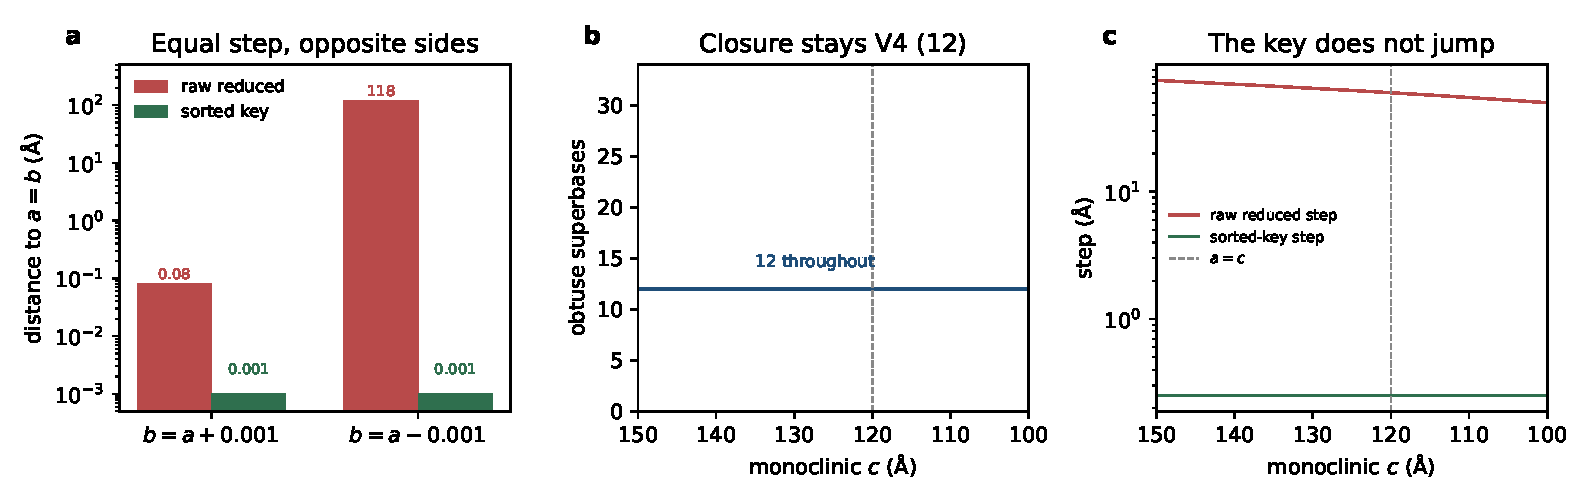
\includegraphics[width=\textwidth]{figures/fig_trajectory.pdf}
\caption{A representative can jump while the sorted key does not. (a) Equal perturbation of $0.001$\,\Ang\ on either side of $a=b$: raw reduced distance $0.080$ versus $118.5$, sorted-key distance $0.0010$ on both sides. (b) Along the monoclinic series the Selling closure stays at 12 superbases through $a=c$. (c) Consecutive raw reduced steps stay tens of angstroms; consecutive sorted-key steps stay near $0.25$\,\Ang.}
\label{fig:trajectory}
\end{figure}

\subsection{Archive search as ordinary computational geometry}
\label{sec:pdb}

Keys were computed for the 206\,214 PDB cells and indexed with a KD tree.\chk{z:timing} On the precomputed keys the index builds in 0.044\,s and a median $k=10$ query takes 0.010\,ms (Python 3.12, NumPy 2.5.3, SciPy 1.18.1). Earlier figures of 0.28\,s and 0.04\,ms are not this measurement. A radius query on that index carries the guarantee of Lemma~\ref{lem:lb}; certification is applied only to the candidates it returns. For scale, the SAUC search of alternate unit cells reported 500-nearest-neighbour queries over roughly half a million PDB and CSD cells in about 4\,s with a Selling embedding versus about 8\,s with Niggli (McGill \emph{et al.}, 2014); those searches operate in an orbit-aware space, whereas a query here searches the lossy key and relies on the certification stage that follows. There is one key per lattice at every Voronoi type;\chk{z:one-key} the extra superbases of symmetric lattices are never inserted into the index and are opened only for certification.

For shape comparison the key is divided by $V^{1/3}$, a neighbourhood graph is built over the whole PDB, and a two-dimensional embedding is drawn. It is an embedding of the key distance, not of Kurlin's complete lattice-isometry space, and nearby points are nearby by construction. The scientific content is in how the observed population occupies the space: when the embedding is coloured afterwards by crystal system, tetragonal populations form branches that approach cubic symmetry at a restricted locus, orthorhombic populations occupy neighbouring and connecting regions, trigonal and hexagonal regions appear at other boundaries, and monoclinic cells spread over a broader area.\chk{z:embedding} None of these labels were used to build the key. Locally, a mean-centred singular-value decomposition of the volume-normalised keys in $k=40$ neighbourhoods, on a 30\,000-cell subsample, gives an entropy effective rank from 1.00 to 5.69, median 2.02.\chk{z:effrank} A previously printed median of 4.12 is not reproduced by this estimator and is not used. The embedding in Fig.~\ref{fig:pdb} is where the population is displayed. The fraction of key-space edges whose distance lies within 10\% of the exact orbit distance has not been reported.\chk{z:audit} Branches and junctions are not read as the global topology of lattice space until that audit is done.

\begin{figure}
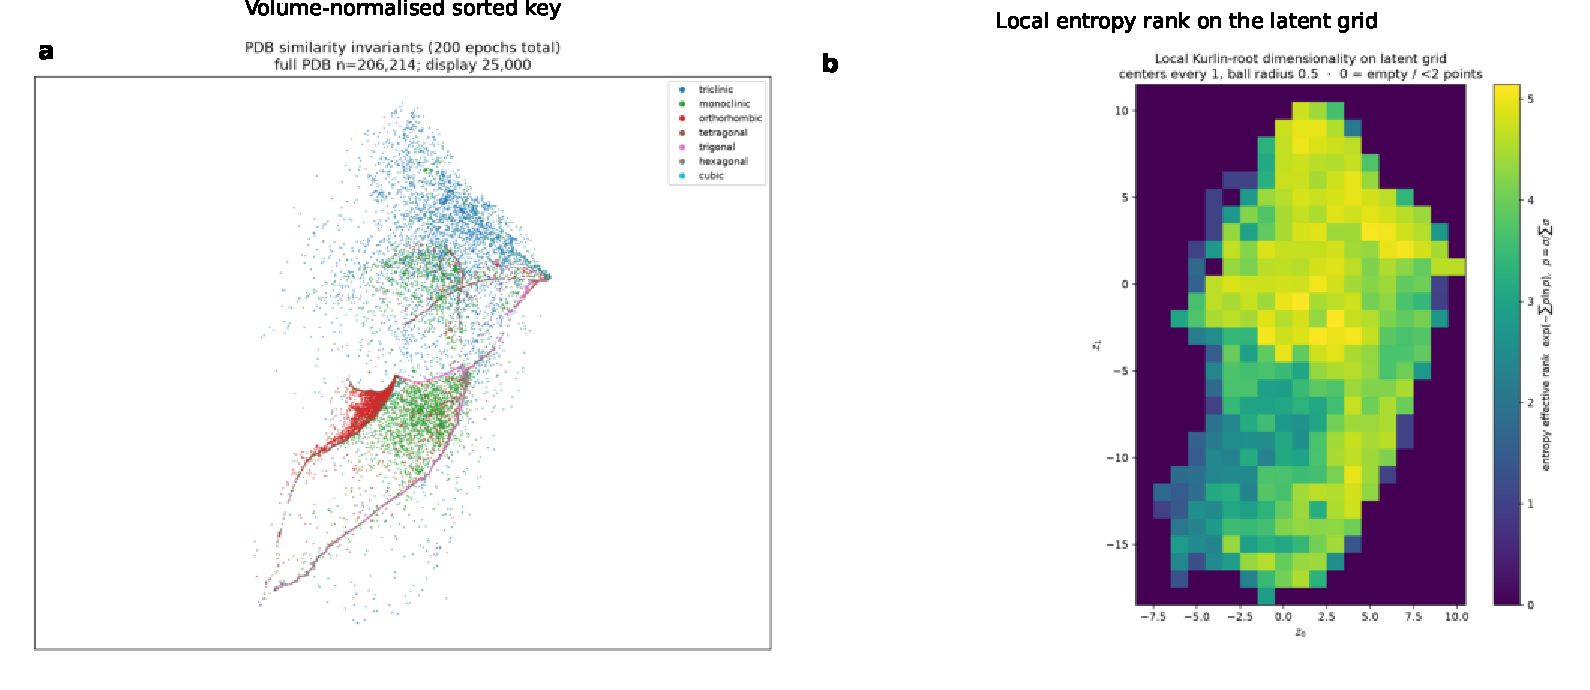
\includegraphics[width=\textwidth]{figures/fig_pdb.pdf}
\caption{Archive shape comparison. (a) Two-dimensional embedding of the volume-normalised sorted key for 206\,214 PDB cells, coloured afterwards by crystal system; 25\,000 cells are drawn. (b) Local entropy effective rank on a unit grid of that latent plane (ball radius 0.5). The neighbourhood estimator cited in the text is a separate $k=40$ calculation in the six-dimensional key, median 2.02, and is not read off panel (b).}
\label{fig:pdb}
\end{figure}

\subsection{An archival protein family as a trajectory}
\label{sec:lysozyme}

The 1361 hen egg-white lysozyme cells span six space groups: 1152 tetragonal $P4_32_12$, 100 orthorhombic $P2_12_12_1$, 59 monoclinic $P2_1$, 41 triclinic $P1$, and small trigonal and hexagonal groups.\chk{z:lysozyme} The key handles all of them in one setting-independent space before any system-specific analysis is chosen. Within the 1113 native-volume tetragonal cells, which span a 26\% range in volume, the leading intrinsic coordinate of the key-distance graph (Fiedler, 1973) correlates with cell shrinkage at $|r|=0.92$: $a$ varies smoothly from about 76.8 to 80.0\,\Ang\ while $c$ stays flat and then steps between preferred values near 37 and 38\,\Ang.\chk{z:lysozyme} For this single-setting subset the same trend could be read directly from $(a,c)$; the gain is that the subset was isolated from a heterogeneous census by one lattice-level distance, after which conventional interpretation proceeds in whatever coordinates suit it.

\subsection{Per-crystal cell variation in a serial XFEL data set}
\label{sec:xfel}

Merged depositions keep only a consensus cell; the CrystFEL stream retains every indexed cell. Because these are unconstrained per-frame cells of a high-symmetry lattice, they are keyed by sorted conorms without the square root (Section~\ref{sec:noise}) and the cloud is analysed by principal components rather than a nonlinear embedding. The $c$ axis has median 233.3\,\Ang, median absolute deviation 0.13\,\Ang, and a maximum of 245\,\Ang. The key is blind to orientation, so orientation metadata can be projected onto the variation as an independent diagnostic (Fig.~\ref{fig:xfel}). Crystals with the beam within $10^\circ$ of $c^*$ ($n=141$) have a $c$-axis median absolute deviation of 0.22\,\Ang, against 0.083\,\Ang\ for beam angles above $80^\circ$ ($n=2866$), a ratio of 2.6.\chk{z:xfel} The earlier scatters of 1.53\,\Ang\ and about 0.5\,\Ang\ are not reproduced under this binning and are not used. The same projection could be made for pulse energy, detector geometry, time delay or temperature without touching the lattice representation.

\begin{figure}
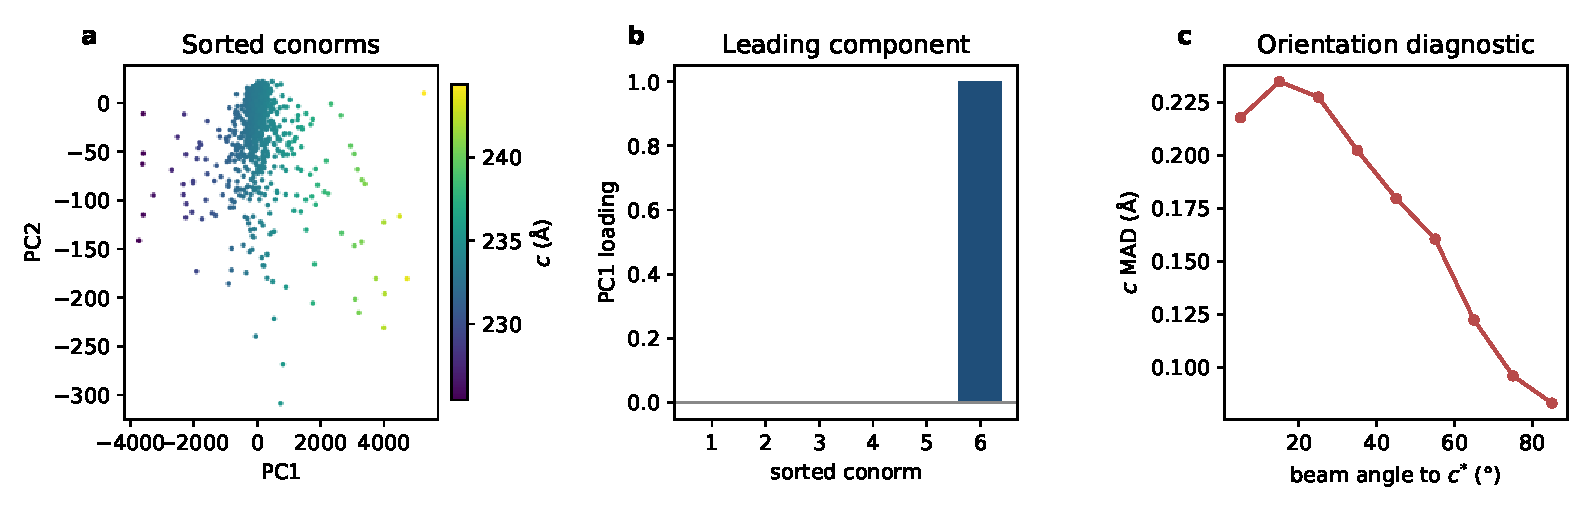
\includegraphics[width=\textwidth]{figures/fig_xfel.pdf}
\caption{Per-crystal cells from CXIDB 83, keyed by sorted conorms. (a) Principal-component scores of 4\,000 crystals, coloured by $c$. (b) Loadings of the leading component, carried by the largest sorted conorm. (c) Median absolute deviation of $c$ against the angle between the beam and $c^*$.}
\label{fig:xfel}
\end{figure}

\subsection{Reindexing: identify the lattice first, then the basis}
\label{sec:reindex}

A conventional reindexing search asks which small integer matrix maps one cell onto another, mixing ``is this the same lattice?'' with ``which basis?''. Here they are separated by the procedure of Section~\ref{sec:reindex-proc}. On an orthorhombic P cell presented in an even-class basis $\{v_1,v_3,v_2-v_1\}$ the procedure returns the full eight-member $mmm$ coset, whereas the 24 relabellings of a single reduced superbase return nothing;\chk{z:coset} on an arbitrary unimodular resetting of a reference cell, with and without noise and centering, it recovers the resetting up to automorphism for eight lattice types.\chk{z:reindex-proc}

On the 200 perturbed monoclinic frames spanning both sides of a reduction flip, a brute-force baseline tested all 6960 unimodular matrices with entries in $\{-1,0,1\}$ per frame. The key-first workflow reduced each frame to a cached two-operator coset, with the reference closure enumerated once before the first frame.\chk{z:reindex-bench} A rerun of that appendix procedure does not recover the earlier wall-clock figures: on this machine the 6960-matrix baseline has median 15\,ms per frame and the cached procedure median 75\,ms per frame. The figures 0.07\,ms per frame and 330-fold are not reproduced and are not used. The baseline is a cost comparison, not a correctness reference. A search over matrices with entries in $\{-1,0,1\}$ finds the relating operator only if that operator has no entry of magnitude two or more; for arbitrary input settings this fails outright, since $\mathrm{GL}(3,\mathbb Z)$ is infinite and most random resettings with entries up to $\pm2$ are invisible to it (192 of 200 in the test).\chk{z:brute-complete} The usual defence is to reduce both cells first. With Niggli reduction the defence works: for two Niggli cells of the same lattice, exact or noisy, in random input settings, every relating operator had entries in $\{-1,0,1\}$ across eight lattice types,\chk{z:brute-complete} consistent with the classical fact that Buerger-cell boundary transformations and point-group operations in a reduced basis are all small. With Selling reduction alone it does not work: two obtuse superbases of the same V3 lattice (rhombic dodecahedron; face-centred lattices) can be related by an operator with an entry of magnitude two,\chk{z:brute-complete} which the small search silently misses. The brute force is therefore complete only conditionally, on a correct Niggli reducer and on an entry bound that holds for reduced bases, whereas the closure route is complete unconditionally, by enumeration, and needs at most 32 candidates rather than 6960.\chk{z:reindex-bench}

\subsection{Reduction flips are recovered exactly, not tolerated as pseudo-symmetry}
\label{sec:flip}

Near a pseudo-symmetric boundary a tolerance-gated symmetry search can drop a basis change that is needed only because reduction picked a different representative. In the controlled monoclinic family, exchanging $a$ and $c$ is an exact integer relation between two settings of the same lattice for every $|a-c|$, but an exact metric symmetry only at $a=c$. With a $3^\circ$ Le~Page tolerance the exchange is admitted up to about $|a-c|=2.85$\,\Ang\ and then excluded, although the two descriptions remain exactly related; raising the tolerance merely admits unrelated pseudo-symmetries. The closure-based operator search recovers the exact exchange regardless of how far the lattice is from symmetric (Table~\ref{tab:flip}).\chk{z:lepage} The same family, with $a=c$ imposed, gives $H^*$ of index 2 over $H$ and recovers the exchange with residual proportional to $|a-c|$ at every distortion; the near-tetragonal cuboid with its two short edges equalized gives index 2 and a four-fold outside $H$.\chk{z:pseudo}

\subsection{Coset size, tolerance and noise on high-symmetry frames}
\label{sec:tolerance}

Matching only one representative per isometry class returns one operator per class pair and loses the coset. On exact cells, an orthorhombic P cell against itself returns the order-8 $mmm$ coset when matched over the full 32-member closure and only 2 operators when matched over representatives; the $P6_3$ cell against itself returns 24 ($6/mmm$ including $-I$) versus 4.\chk{z:coset} Too tight a verification tolerance lets noise select a subset of the coset: on $P6_3$ frames with $0.05^\circ$ angular noise, a relative tolerance of $10^{-4}$ returned 12 of the 24 operators and $10^{-3}$ returned all 24.\chk{z:verify-tol} With exact zero detection a measured $P6_3$ frame is classified as V1 and only the 24 relabellings of one superbase are matched; widening the zero tolerance to a few $\sigma$ on the invariant scale of Appendix~C restores the V4 classification and the full closure, and two independently perturbed frames at $0.01^\circ$ and $0.05^\circ$ angular noise then both recovered all 24 operators.\chk{z:noisy-frames}

%==============================================================================
\section{Discussion}
%==============================================================================

\subsection{The problem changed, so the object changed}

Reduction methods are sometimes compared as competing answers to one question. It is more useful to see them as answers to different questions. The classical question --- which cell should represent this lattice? --- is answered well by Niggli reduction, and its seams are the unavoidable price of picking one representative. The modern question --- which lattice is this, which lattices are near it, and only then which basis is needed? --- is better served by a finite closure for the exact part and a coarse continuous key for the search part. The order of computation is: enter primitive lattice space; build the closure appropriate to the Voronoi type; retrieve with one key per lattice; certify candidates over the full closure; propagate the exact operator to the data that need it. This complements Niggli reduction; it does not replace it.

\subsection{A lower-bound key is enough}

Lattice-isometry space has not been equipped with a Euclidean metric here; Kurlin (2026) explicitly postpones that construction. What is available is weaker and sufficient: a lossy key whose distance is a lower bound on the true one, which is exactly what a certified filter needs. The exploratory tools that run on the key --- nearest neighbours, principal components, embeddings --- are descriptive, and their validation is done upstream by auditing key collisions and graph edges against exact comparisons.

\subsection{Which tolerances remain, and what they decide}

The Le~Page-style bet --- that an exact integer relation between two settings is found only if it lies inside a symmetry group enlarged by an angular tolerance --- is gone, because the closure search is finite and complete. Two tolerances remain, of different kinds. The closure tolerance decides which conorms count as zero for enumeration; being generous costs at most a few extra candidates, each of which is verified, so it is set well above the noise and is not a bet. The verification tolerance decides whether two metrics are the same lattice and, on a symmetry stratum, which automorphisms count. This is the indexing ambiguity itself, which no geometry resolves; it is calibrated on a linear residual from known same- and different-lattice pairs, and the safe direction is to accept the whole coset and pass it to intensity statistics. Pseudo-symmetry, when wanted, is a declared distance to a stratum rather than a per-operator angular gate.

\subsection{Continuity does not abolish crystal systems}

Higher-symmetry lattices sit on lower-dimensional loci of lattice space where extra metric equalities hold and extra automorphisms appear. The PDB population is naturally read as a continuous object stratified by these familiar discrete classes, and a trajectory may approach, cross or leave a stratum. A representation built around one canonical cell makes such transitions look like jumps in description; a lattice-level coordinate lets the physical path and the changing set of exact basis correspondences be handled separately.

\subsection{Scope and attribution}

Three objects must stay distinct: Kurlin's structured root form, which is the complete isometry classification; the sorted key, which is continuous and Euclidean but many-to-one; and the exact operator test over the closure, which establishes identity. No claim here requires one object to be all three. The framework addresses equality, similarity and basis equivalence of primitive lattices; supercell and subcell relations change the lattice and need explicit enumeration of finite-index sublattices when they are part of the search problem.

%==============================================================================
\section{Conclusions}
%==============================================================================

A century of reduction practice has rightly emphasized the question of which cell should represent a lattice. Large-scale computation is better served by asking first which lattice this is and which are near it, and only then which basis is needed. Selling reduction provides the finite object between those questions; sorting its root products provides a continuous Euclidean key whose distance is a safe lower bound; exact integer algebra over the Selling closure provides the reindexing operator and its coset. In one line: Euclidean key, then finite Selling closure, then exact operator.

%==============================================================================
\appendix
%==============================================================================

\section{Selling reduction and the Selling closure}
\label{app:closure}

\subsection{Superbase, conorms, vonorms}
Given a primitive basis $v_1,v_2,v_3$, set $v_0=-(v_1+v_2+v_3)$. The four vectors form a superbase. Their six conorms are $p_{ij}=-v_i\cdot v_j$ for $0\le i<j\le3$. In the $S^6$ convention of Andrews \emph{et al.} (2019) the Selling scalars are $s_{ij}=-p_{ij}$ and occupy the non-positive orthant; everything below is written in conorms. The seven vonorms (Conway \& Sloane, 1992) are the squared lengths of the four vectors and of the three opposite-edge partial sums,
\begin{equation}
v_i^2=\sum_{j\ne i}p_{ij},\qquad v_{ij}^2=(v_i+v_j)^2=p_{ik}+p_{il}+p_{jk}+p_{jl},
\end{equation}
with $\{k,l\}=\{0,1,2,3\}\setminus\{i,j\}$; they satisfy $v_0^2+v_1^2+v_2^2+v_3^2=v_{01}^2+v_{02}^2+v_{03}^2$ and are the $D_7$ descriptor of Andrews and Bernstein and Kurlin's voform.

\subsection{Reduction}
A superbase is obtuse if all $p_{ij}\ge0$. If some $p_{ij}=-\varepsilon<0$, the Delone--Selling move replaces the superbase by
\begin{equation}
u_i=-v_i,\quad u_j=v_j,\quad u_k=v_i+v_k,\quad u_l=v_i+v_l,
\end{equation}
which keeps the zero sum, generates the same lattice, permutes six of the seven vonorms and decreases the seventh by $4\varepsilon$; the sum of the six conorms decreases by $\varepsilon$ (Kurlin, 2026, Lemma~A.1).\chk{z:reduction-step} Applying the move to the most negative conorm until none remains terminates in finitely many steps.\chk{z:reduction-step} This is the algorithm of Andrews \& Bernstein (1988, 2014) and Andrews \emph{et al.} (2019); the conventional-to-primitive conversion that precedes it is the only rational step, and all subsequent operations are integer unimodular.

\subsection{The closure}
Relabelling the four vectors of an obtuse superbase ($S_4$, 24 elements) and negating all of them always gives obtuse superbases of the same lattice. Kurlin's Lemmas~4.1--4.5 show that these are all of them only for lattices whose Voronoi cell is the generic truncated octahedron (V1). For the four degenerate types there are additional obtuse superbases not related by relabelling, obtained from the reduced one by the move above applied at a conorm that is exactly zero. Table~\ref{tab:closure} lists the counts; they were confirmed by exhaustive enumeration of all obtuse superbases with bounded integer coordinates for one test lattice of each type.\chk{z:closure-count} The Voronoi type is read directly from the zero pattern of the reduced conorms: no zeros is V1; one is V2; two on opposite tetrahedral edges is V3; two sharing a vertex is V4; three is V5, and other three-zero patterns cannot occur.\chk{z:type-rule} For a symmetric lattice within a type the classes may coincide (the hexagonal lattice has one class rather than three, because its automorphisms relate them); the enumeration handles this automatically.\chk{z:closure-count}

For measured cells, a conorm that is exactly zero in the ideal lattice is a small positive or negative number, so the closure enumeration must treat conorms within a noise tolerance of zero as zero. The tolerance is set from the angular noise model of Appendix~C on the closure-invariant scale $T$ defined there.

\section{The sorted key: invariance, continuity, lower bound, collisions}
\label{app:key}

\subsection{One key per lattice}
Relabelling permutes the six conorms, so the sorted list is unchanged, and central inversion leaves every conorm unchanged. For the additional closure members at V2--V5, Kurlin's Lemmas~4.2--4.5 give the coform of each alternative superbase explicitly as a transposition or permutation of the conorms of the reduced one; hence the multiset of conorms is the same on every member of the closure, and so is $\sortkey$. This is the modern form of the classical statement that the reduced Selling scalars are unique as a list (Bravais, 1850; Delone, 1932; Andrews \emph{et al.}, 2019). Numerically, the 4, 6, 12 and 32 superbases of the V2--V5 test lattices each gave a single sorted key.\chk{z:one-key}

\subsection{Continuity}
Sorting is 1-Lipschitz. Kurlin's Lemma~6.6 bounds the change of each root product under a basis perturbation of size $\delta$ by $\sqrt{2\ell\delta}$, where $\ell$ bounds the vector lengths. Across a Voronoi-type boundary the reduction may return a superbase near a different closure member, but all members share the limiting key, so the lattice-level key is continuous through the boundary, with the H\"older-$\tfrac12$ rate of Appendix~C at the symmetry strata themselves.\chk{z:trajectory}

\subsection{Proof of Lemma~\ref{lem:lb}}
Expanding $\|x-\sigma y\|_2^2=\|x\|^2+\|y\|^2-2\langle x,\sigma y\rangle$, the minimum over $\sigma$ is attained when $\langle x,\sigma y\rangle$ is maximal, which by the rearrangement inequality occurs when both vectors are similarly ordered; that value is $\langle\sort x,\sort y\rangle$. The inequality holds because $G\subseteq S_6$.\chk{z:lowerbound} The physically realisable relabellings of the six conorms form the image of $S_4$ in $S_6$, a subgroup of order 24, so the lemma applies with $G$ that image: the key distance is a lower bound on the orbit distance and the tightest lower bound available from the unpaired multiset alone. The same argument applies verbatim to any monotone per-slot transform of the conorms (Appendix~C), provided the transform depends only on the conorm and on lattice invariants.

\subsection{Why the key is Euclidean and the orbit metric is not}
The lemma identifies the key distance with the quotient metric of $\mathbb R^6$ by $S_6$ acting by coordinate permutations. $S_6$ is generated by the transpositions $(i\,j)$, each the reflection in the hyperplane $x_i=x_j$; for a finite reflection group the quotient $\mathbb R^n/W$ is isometric to a closed Weyl chamber, here the convex cone $\{s_1\le s_2\le\dots\le s_6\}$, with the metric inherited from $\mathbb R^n$. Convexity makes chordal and intrinsic distance agree, so the key space is a flat Euclidean domain. The image of $S_4$ in $S_6$ contains no reflection: a transposition of two vertices moves two pairs of edges, which is a rotation in $\mathbb R^6$. Its quotient is an orbifold with singular strata, not a convex cone, and the orbit metric $\min_{\sigma\in S_4}\|x-\sigma y\|$ is not Euclidean-embeddable, as Schoenberg's criterion confirms numerically.\chk{z:euclid} This is the obstruction that Kurlin's deferred metric on the root-invariant space must address; the sorted key sidesteps it by quotienting by the larger reflection group, at the price of the collisions counted next.

\subsection{Collisions}
The sorted key forgets the pairing of conorms into the three opposite-edge columns of Kurlin's $2\times3$ root form. For six distinct values the $S_4$-orbit of a labelled coform has 24 elements and there are $6!=720$ arrangements, so $720/24=30$ non-isometric lattices share a generic V1 key. The same count gives 15 for V2 ($5!/|D_4|$) and 4 for V4 (which of four values is the distinguished one); V3 and V5 are injective. Concretely, the coforms $\begin{pmatrix}1&2&3\\4&5&6\end{pmatrix}$ and $\begin{pmatrix}1&2&3\\4&6&5\end{pmatrix}$ are non-isometric lattices with identical keys.\chk{z:fibre}

\subsection{A sharper key}
Kurlin's Example~6.5 exhibits non-isometric lattices with identical vonorm multisets ($D_7$ alone is incomplete) but different conorm multisets, which the sorted key separates. The converse also holds empirically: in 300 random generic V1 fibres, all 30 lattices sharing a sorted key had distinct sorted-$\sqrt{D_7}$ keys.\chk{z:d7} The concatenated key $\sort(r)\,\|\,\sort(\sqrt{\text{vonorms}})\in\mathbb R^{13}$ is still a pure sort, still continuous, still satisfies Lemma~\ref{lem:lb} blockwise, and reduces the generic over-retrieval to essentially one. This is an observation rather than a theorem; ties and degenerate types need separate treatment, and the six-dimensional key remains the archival key of this paper.

\section{Noise: the H\"older-$\tfrac12$ cusp and how to remove it}
\label{app:noise}

\subsection{The effect}
Angular measurement error is approximately Gaussian in conorm space, because $p_{ij}$ is linear in the metric tensor: $\sigma_{p_{ij}}\approx|v_i||v_j|\sigma_\theta$.\chk{z:noise} The square root maps this to the key. Where $p>0$ the map is locally linear with slope $1/(2\sqrt p)$; where $p=0$ it satisfies only $|\sqrt x-\sqrt y|\le\sqrt{|x-y|}$, so the response to noise is proportional to $\sqrt{\sigma_p}$ rather than to $\sigma_p$. Every lattice with a right angle in its obtuse superbase has such a zero. On the $P6_3$ cell $(41.8,41.8,233,90,90,120)$ the numbers are in Table~\ref{tab:noise}: a $0.01^\circ$ error moves the plain key by a median 1.58\,\Ang, while the same error on a generic triclinic cell moves it by roughly 0.03\,\Ang.\chk{z:noise}

\subsection{Stabilized keys}
Any monotone per-slot map $f$ applied to the conorms before sorting preserves one-key-per-lattice and Lemma~\ref{lem:lb} in the transformed metric, provided $f$ depends only on $p$ and on lattice invariants. The noise floor $s$ used below must therefore be closure-invariant. Per-pair floors $|v_i||v_j|\sigma_\theta$ are not: the even-class superbases of a cuboid have different edge lengths, and keys computed from two bases of the same cuboid then differ by about 0.02\,\Ang.\chk{z:floor-invariance} A suitable invariant scale is
\begin{equation}
T=\sum_{i<j}p_{ij}=\tfrac12\sum_i|v_i|^2 ,
\end{equation}
which the Selling move at a zero conorm leaves unchanged because it permutes the conorms;\chk{z:floor-invariance} the floor is $s=\sigma_\theta T$. Three options, in increasing order of aggressiveness, are the floored root $\sqrt{p+s}-\sqrt s$, which equals $\sqrt p$ for $p\gg s$ and is linear with slope $1/(2\sqrt s)$ for $p\ll s$, so that the key becomes Lipschitz while staying smooth, monotone and in length units; the soft threshold $\sqrt{\max(p-\kappa s,0)}$, a positive-part shrinkage onto the symmetry stratum with the largest noise reduction, deliberately blind to deviations from symmetry below $\kappa\sigma_p$; and the linear key $\sort(p)$ or $\sort(p/\sqrt T)$, with no square root, which is Lipschitz and Gaussian-noise preserving and is the natural choice for per-frame principal-component analysis. Table~\ref{tab:noise} gives their measured behaviour.\chk{z:stabilise} A stabilized key is a different metric from Kurlin's: choosing $s$ chooses the resolution below which ``symmetric'' and ``nearly symmetric'' are no longer distinguished, and Lemma~\ref{lem:lb} then holds in the stabilized metric.

\section{Exact certification, cosets and pseudo-code}
\label{app:exact}

\subsection{Operator construction}
During reduction the four superbase vectors are tracked as integer coordinate triples in the input primitive basis, for every member of the closure. For a candidate pair $(A,B)$ let $\Uop(A)$ and $\Uop(B)$ be $3\times3$ integer matrices whose columns are three of the four vectors of a superbase from $\Sclosure(A)$ and $\Sclosure(B)$ respectively, under one of the 24 relabellings and one sign. Any three vectors of a zero-sum superbase form a primitive basis, so both matrices are unimodular and $\Pop=\Uop(A)\Uop(B)^{-1}$ is an exact integer matrix. It is accepted if $\Pop^{\mathsf T}\Gmet(A)\Pop=\Gmet(B)$ to within a residual tolerance $\max(\texttt{verify\_abs},\ \texttt{verify\_rel}\cdot\tr|\Gmet(B)|)$. The residual is linear in the metric, so its noise model is Gaussian with scale $\sigma_p$; no square root is involved at this stage. Equivalently, if the rows of $A$ are the integer coordinates of three superbase vectors of $R$ in $\Bbasis_R$ and the rows of $B$ those of the corresponding vectors of $N$ in $\Bbasis_N$, the two vector triples coincide in space exactly when $\Bbasis_RA^{\mathsf T}=\Bbasis_NB^{\mathsf T}$, so $\Pop=A^{\mathsf T}B^{-\mathsf T}$ with both factors unimodular.

\subsection{The procedure as pseudo-code}
\begin{small}\begin{verbatim}
PREPARE_REFERENCE(R_conv, sigma_theta):       # run once, cache the result
  C_R, G_R <- centering matrix and primitive metric of R   # rational C_R
  U_R      <- selling_reduce(G_R)   # 4x3 integer rows, obtuse superbase
  tau      <- 3 * sigma_theta * T(G_R) / 6      # invariant zero tolerance
  S_R      <- closure(U_R, G_R, tau)  # ALL obtuse superbases, <= 32
  key_R    <- sort(sqrt(conorms(U_R, G_R)));  radius <- from sigma (App. C)
  H        <- REINDEX_FRAME(ref, R_conv)   # automorphism coset, = Aut(R)
  if space group known: L <- Laue group;
      branches <- one representative per coset of L in H   (exact H only)
  return ref = (C_R, G_R, U_R, S_R, key_R, radius, H)

REINDEX_FRAME(ref, N_conv, sigma_theta):      # per frame
  C_N, G_N <- centering matrix and primitive metric of N
  if |key(G_N) - ref.key_R| > ref.radius: return EMPTY   # optional screen
  U_N <- selling_reduce(G_N)
  S_N <- closure(U_N, G_N, tau)   # usually {U_N}; larger near a stratum
  ops <- {}
  for C_R' in ref.S_R, C_N' in S_N, pi in S4, eps in {+1,-1}:
      A <- rows 1..3 of eps*C_R'[pi];  B <- rows 1..3 of C_N'
      P <- A^T B^{-T}                 # Bprim_N = Bprim_R P ; integer, |det|=1
      if || P^T ref.G_R P - G_N || <= tol(sigma): ops <- ops + {P}
  ops <- deduplicate(ops)             # = P0 * ref.H ; report (P0, H), by det
  if ref.branches: report (P0, ref.branches)   # |H|/|L| alternatives
  # x_R = P x_N ; h_R = P^{-T} h_N ; W_R = P W_N P^{-1} ; P_conv = C_R P C_N^{-1}
  return ops
\end{verbatim}\end{small}

\subsection{Pseudo-symmetry by closure cosets}
\begin{small}\begin{verbatim}
PSEUDO_SYMMETRY(ref, delta):           # once per reference; delta in conorm units
  cf <- coform(ref.U_R, ref.G_R)       # 2x3 conorms, integer coords retained
  H  <- ref.H                          # exact Aut(R) from the closure self-match
  patterns <- degeneration patterns of cf:      # finite list
      zero sets   {p_ij : p_ij < delta}
      equal sets  {(p_ij, p_kl) : |p_ij - p_kl| < delta}, extended to
                  Aut(R)-orbits, and their unions (closed under Aut(R))
  out <- {}
  for pat in patterns:
      cf* <- impose(pat, cf)           # zero / average whole orbits
      d   <- |cf - cf*|;  if d > delta: continue
      G*  <- Gram from cf* (Kurlin Lemma 6.2), same superbase coordinates
      S*  <- closure(ref.U_R, G*, tau);  H* <- self-match of G* over S*
      assert H subset H*
      for P in H* \ H: residual(P) <- |P^T ref.G_R P - ref.G_R|
      out <- out + {(pat, d, cosets H*/H, cosets H*/L, residuals)}
  return out                           # cached with ref
\end{verbatim}\end{small}
The imposition step must act on whole $\mathrm{Aut}(R)$-orbits of coform entries; otherwise $R^*$ depends on which member of the orbit was edited and $H\subseteq H^*$ can fail.\chk{z:pseudo} The checks reported with this paper do not execute the pattern loop. They impose two strata by hand, as stated in Section~\ref{sec:pseudo}: $a=c$ on the monoclinic family, and equal short edges on the near-tetragonal cuboid.

\subsection{Relation to the Le~Page route}
Le~Page's algorithm finds lattice directions $[uvw]$ and planes $(hkl)$ that are parallel to within $\delta$, that is, approximate twofold axes of $\Gmet$, and assembles the metric point group from them; reindexing operators are then taken from that group, and two settings are related only if the relating operator happens to be a member. This is the right construction for pseudo-symmetry and is unsuited to recovering the operator relating two settings: that operator is exact for every distortion, but its twofold residual grows linearly with the distortion and leaves the gate (Table~\ref{tab:flip}). The closure procedure asks whether $\Pop$ carries $\Gmet(R)$ to $\Gmet(N)$ rather than whether $\Pop$ is a near-symmetry of $\Gmet(R)$, and it is complete because every obtuse superbase of each lattice is on the list. The exact automorphism group is obtained as the self-match; near-automorphisms, when wanted, remain a tolerance-based search for which the twofold method is appropriate.

\subsection{Relation to Lebedev's coset reduction}
Lebedev \emph{et al.} (2006) reduce the operators that intensity statistics must examine to coset representatives of the Laue group $L$ in the lattice symmetry group $H$. For index 2 the non-trivial coset always contains a twofold; for higher index it need not (the coset $\{4,4^3\}$ of $2$ in $422$ contains none), so representatives are chosen of minimal order.\chk{z:coset-reps} Their $H$ is obtained from a tolerance search on the metric, which is appropriate for the pseudo-merohedral case they address. Here $H=\mathrm{Aut}(R)$ is obtained exactly by matching the reference against itself over its cached closure, and the coset argument applied to that exact $H$ reduces the ambiguity handed to intensities from $|H|$ operators to $|H|/|L|$ branches, computed once per reference. If pseudo-merohedral branches are wanted, the same coset argument is applied to the tolerance-enlarged $H^*$ of Section~\ref{sec:pseudo} in a separate, declared step.

\subsection{Completeness of the closure route versus a bounded unimodular search}
The closure route is complete because every obtuse superbase of each lattice is enumerated (Kurlin, 2026, Lemmas~4.1--4.5) and the reduction bookkeeping absorbs whatever large integers the input bases carried; no bound on the entries of $\Pop$ is assumed, and entries of magnitude two, which occur in V3, are produced rather than searched for. A search over unimodular matrices with entries in $\{-1,0,1\}$ is complete only under an entry bound. That bound holds empirically between Niggli cells of one lattice (exact or noisy, any input setting) but not between Selling-reduced settings of a V3 lattice.\chk{z:brute-complete} Niggli-first therefore makes the small search correct, at the price of reintroducing the representative's boundary behaviour as an implementation dependency and of testing 6960 candidates where the closure needs at most 32. The implementation of the Niggli change-of-basis must itself be verified: the returned matrix $N$ should satisfy $N^{\mathsf T}\Gmet N=\Gmet_{\rm red}$ exactly, and this identity belongs in the test suite.\chk{z:brute-complete}

\subsection{If nothing is accepted}
Either $N$ is a different lattice; or $N$ is a sub- or supercell of $R$ (a different lattice, requiring finite-index enumeration outside this procedure); or the tolerance is tighter than the noise. The residual of the best-scoring candidate is reported in all cases, so the third possibility is visible rather than silent.

%==============================================================================
\section*{Data and code availability}
The cell key, lattice comparison, reindexing coset and PDB radius search are library calls in \texttt{agentsg.cell} and, unchanged, on a local read-only service (\texttt{agentsg.serve}), whose REST endpoints are \texttt{GET /v1/cell}, \texttt{POST /v1/compare}, \texttt{POST /v1/reindex} and \texttt{POST /v1/pdb/search}; the same four calls are exposed as MCP tools. Space-group, reflection, site and plate tools served by the same process are outside the scope of this paper. The source is \texttt{https://github.com/phzwart/agentsg}. An archival DOI for that repository has not been minted. The 206\,214 PDB cells used for the index are the snapshot \texttt{https://doi.org/10.5281/zenodo.22986222}. Lysozyme cells derive from public PDB entries (UniProt P00698). Serial data are CXIDB entry 83 (DOI 10.11577/1464102), the $\beta$-lactamase stream of Wiedorn \emph{et al.} (2018). The Supporting Information lists, for every marked statement, the computation that checks it.

\ack{This work was carried out in the Molecular Biophysics and Integrated Bioimaging Division, Lawrence Berkeley National Laboratory. No grant or contract number is recorded in the project sources.}

%==============================================================================
\begin{references}
\reference{Andrews, L. C. \& Bernstein, H. J. (1988). \emph{Acta Cryst.} A\textbf{44}, 1009--1018.}
\reference{Andrews, L. C. \& Bernstein, H. J. (2014). \emph{J. Appl. Cryst.} \textbf{47}, 346--359.}
\reference{Andrews, L. C. \& Bernstein, H. J. (2016). \emph{J. Appl. Cryst.} \textbf{49}, 756--761.}
\reference{Andrews, L. C. \& Bernstein, H. J. (2023). \emph{Acta Cryst.} A\textbf{79}, 485--498.}
\reference{Andrews, L. C., Bernstein, H. J. \& Sauter, N. K. (2019). \emph{Acta Cryst.} A\textbf{75}, 593--599.}
\reference{Bravais, A. (1850). \emph{J. \'Ec. Polytech.} \textbf{19}, 1--128.}
\reference{Brehm, W. \& Diederichs, K. (2014). \emph{Acta Cryst.} D\textbf{70}, 101--109.}
\reference{Bright, M., Cooper, A. I. \& Kurlin, V. (2021). arXiv:2109.11538.}
\reference{Conway, J. H. \& Sloane, N. J. A. (1992). \emph{Proc. R. Soc. London Ser. A}, \textbf{436}, 55--68.}
\reference{Delone, B. N. (1932). \emph{Z. Kristallogr.} \textbf{84}, 109--149.}
\reference{Fiedler, M. (1973). \emph{Czech. Math. J.} \textbf{23}, 298--305.}
\reference{Gildea, R. J. \& Winter, G. (2018). \emph{Acta Cryst.} D\textbf{74}, 405--410.}
\reference{Grosse-Kunstleve, R. W., Sauter, N. K. \& Adams, P. D. (2004). \emph{Acta Cryst.} A\textbf{60}, 1--6.}
\reference{Kurlin, V. (2026). \emph{A complete isometry classification of 3-dimensional lattices.} Revised manuscript, April 2026. https://kurlin.org/projects/lattice-geometry/lattices3Dmaths.pdf.}
\reference{Lebedev, A. A., Vagin, A. A. \& Murshudov, G. N. (2006). \emph{Acta Cryst.} D\textbf{62}, 83--95.}
\reference{Le Page, Y. (1982). \emph{J. Appl. Cryst.} \textbf{15}, 255--259.}
\reference{McGill, K. J., Asadi, M., Karakasheva, M. T., Andrews, L. C. \& Bernstein, H. J. (2014). \emph{J. Appl. Cryst.} \textbf{47}, 360--364.}
\reference{Niggli, P. (1928). \emph{Krystallographische und strukturtheoretische Grundbegriffe.} Handbuch der Experimentalphysik, Vol.~7, Part~1. Leipzig: Akademische Verlagsgesellschaft.}
\reference{Wiedorn, M. O. \emph{et al.} (2018). \emph{Nature Commun.} \textbf{9}, 4025.}
\end{references}

%==============================================================================
% TABLES
%==============================================================================

\begin{table}
\caption{The Selling closure by Voronoi type (Kurlin, 2026, Lemmas 4.1--4.5). ``Classes'' are families of obtuse superbases not related by relabelling; the group in parentheses is the relabelling ambiguity remaining inside the coform once the zero pattern is fixed: $S_4$ on all six conorms (V1), $D_4$ on the $2\times2$ nonzero block (V2), $S_4$ on the four nonzero conorms (V3), $S_3$ on three conorms with one fixed (V4), and the three nonzero conorms free (V5). ``Zeros'' is the number of zero conorms in the reduced superbase, ``fibre'' the generic number of non-isometric lattices sharing one sorted key. Superbases are counted as unordered sets of four vectors, so a generic lattice contributes two (the superbase and its global negation).}
\label{tab:closure}
\begin{footnotesize}\begin{tabular}{llcccc}
type & Voronoi cell & zeros & superbases & classes (group) & fibre \\
\hline
V1 & truncated octahedron & 0 & 2 & 1 ($S_4$) & 30 \\
V2 & hexa-rhombic dodecahedron & 1 & 4 & 2 ($D_4$) & 15 \\
V3 & rhombic dodecahedron & 2, opposite & 6 & 3 ($S_4$) & 1 \\
V4 & hexagonal prism & 2, at a vertex & 12 & 3 ($S_3$) & 4 \\
V5 & cuboid & 3 & 32 & 4 (free) & 1 \\
\end{tabular}\end{footnotesize}
\end{table}

\begin{table}
\caption{Four sources of ambiguity in assigning indices, and where each is resolved.}
\label{tab:ambiguity}
\begin{small}\begin{tabular}{p{2.1cm}p{3.6cm}p{4.2cm}p{2.1cm}}
ambiguity & what it is & resolved by & tolerance \\
\hline
setting & same lattice, different cell (bookkeeping) & closure and metric test: unique $\Pop_0$ modulo $H$ & noise residual only \\
exact symmetry & $H=\mathrm{Aut}(R)$ modulo Laue group $L$ & intensities, or carried as $H/L$ & none \\
pseudo-symmetry & automorphisms of a nearby lattice, $H^*\supset H$ & Section~\ref{sec:pseudo}; intensities over $H^*/L$ & one declared distance \\
key collision & different lattices, same sorted key & certification stage & none \\
\end{tabular}\end{small}
\end{table}

\begin{table}
\caption{Monoclinic axis exchange under increasing distortion. The two settings describe the same lattice throughout. A $3^\circ$ pseudo-symmetry gate eventually drops the exchange; closure-based recovery returns the exact integer operator at every distortion.}
\label{tab:flip}
\begin{tabular}{cccccc}
$|a-c|$ (\Ang) & flip $\delta$ ($^\circ$) & key dist. & $\delta$-gate & exact op. & residual \\
\hline
0.0  & 0.00  & $0$ & keeps & yes & $0$ \\
1.0  & 1.04  & $7\times10^{-15}$ & keeps & yes & $0$ \\
2.0  & 2.09  & $2\times10^{-14}$ & keeps & yes & $0$ \\
2.85 & 2.98  & $7\times10^{-15}$ & keeps & yes & $0$ \\
4.0  & 4.18  & $1\times10^{-14}$ & drops & yes & $0$ \\
5.0  & 5.22  & $2\times10^{-14}$ & drops & yes & $0$ \\
10.0 & 10.41 & $7\times10^{-15}$ & drops & yes & $0$ \\
\end{tabular}
\end{table}

\begin{table}
\caption{Median key shift (\Ang) under Gaussian angular noise on the $P6_3$ cell $(41.8,41.8,233,90,90,120)$; invariant floor $s=\sigma_\theta T$, soft threshold $\kappa=2$, linear key $p/\sqrt T$.}
\label{tab:noise}
\begin{tabular}{ccccc}
$\sigma_\theta$ & $\sqrt p$ & $\sqrt{p+s}-\sqrt s$ & $\sqrt{\max(p-2s,0)}$ & $p/\sqrt T$ \\
\hline
$0.01^\circ$ & 1.58 & 0.28 & 0.03 & 0.01 \\
$0.05^\circ$ & 3.12 & 0.64 & 0.17 & 0.06 \\
$0.10^\circ$ & 4.63 & 0.68 & 0.35 & 0.10 \\
\end{tabular}
\end{table}

\end{document}                    % DO NOT DELETE THIS LINE
